
\subsection{Virtual Closed-Loop Prosthesis}
 
Investigating the usability of the two sensory configurations in a closed-loop scenario required these to be interfaced with a prosthetic device, which accommodated the actuation of rotational and hand aperture DoF's. However, using a real prosthesis might result in auditory feedback being provided to the subject through prosthetic actuation sounds, eliminating the interest of solely exploring the impact of tactile feedback. Furthermore, simulating a virtual prosthesis would likely eliminate the output delay caused by motor actuation in a real prosthesis. Hence, it was chosen to simulate a velocity-based virtual prosthesis which enabled evaluation of the developed feedback schemes. In figure \ref{fig:pa:gridmap} is a depiction of a grid system, where the axes corresponded to the wrist rotation and hand aperture. The grid squares represented the discrete feedback variable intervals, and the cursor represented the current position state.  
\begin{figure}[H]                 
	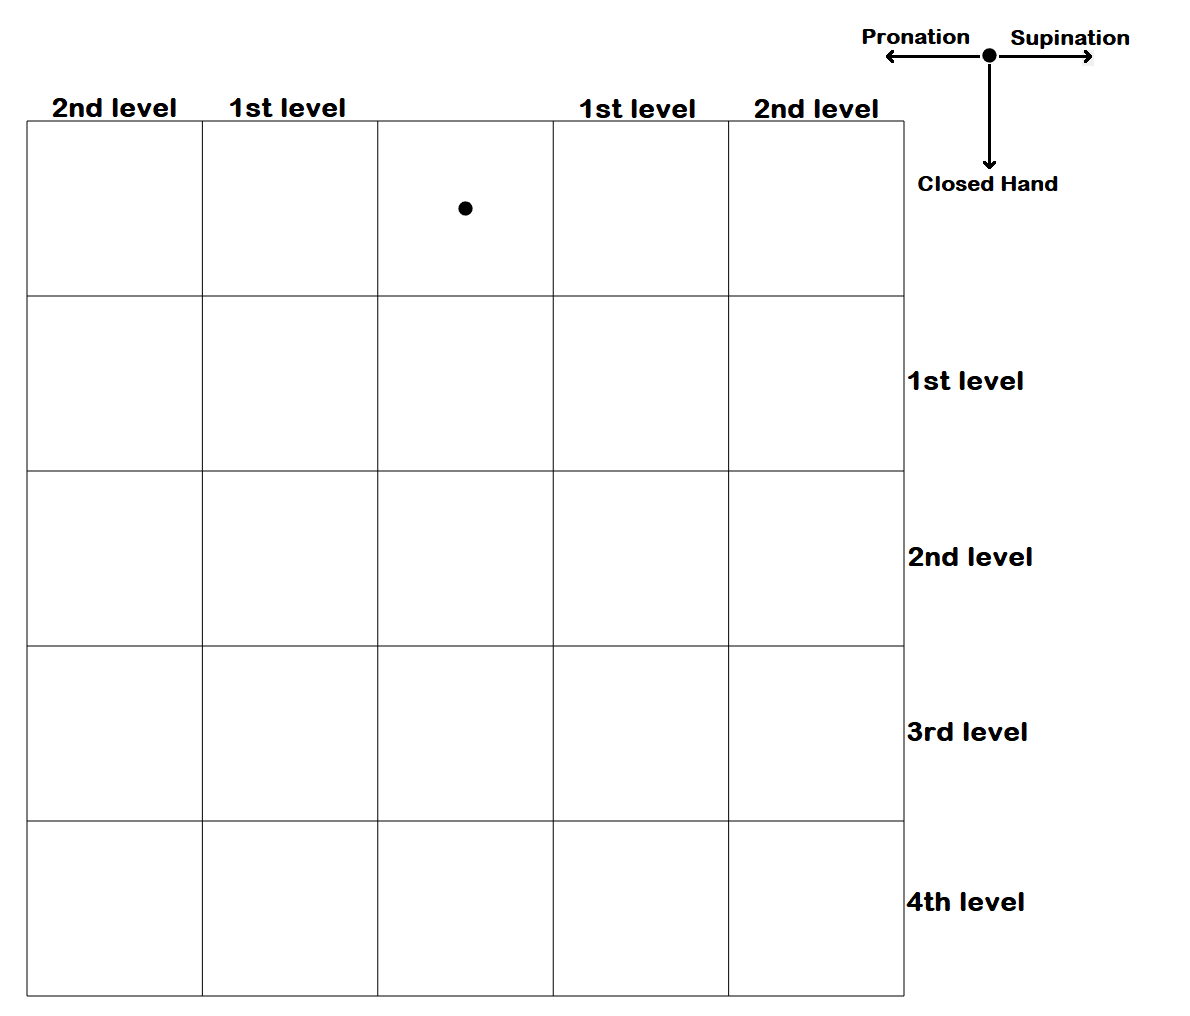
\includegraphics[width=1\textwidth]{figures/gridmap2}  
	\caption{Image of the grid map and cursor used to indicate feedback variable intervals and to simulate the position states of a prosthesis, respectively. Wrist supination moved the cursor to the right, pronation moved it to the left and closing the hand moved it downwards. For left-handed subjects, the rotational movements were reversed. Opening the hand moved the cursor upwards, and was used as a correction movement if needed.}
	\label{fig:pa:gridmap} 
\end{figure}
\begin{figure*}[h]
	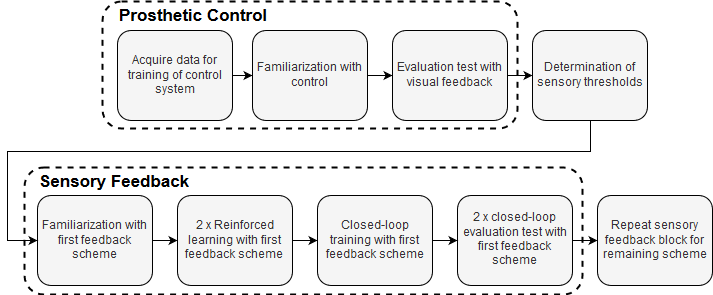
\includegraphics[width=.85\textwidth]{figures/std_paper}
	\caption{Pipeline showing the stages of the experiment. The stages in the first block focused on developing a prosthetic control system, and evaluating the subjects' ability to control the prosthesis. Then stimulation threshold levels were determined. The second block focused on training the understanding of the feedback schemes and evaluating their usability in combination with prosthetic control. The electrotactile feedback block was repeated for the remaining feedback scheme.}
	\label{fig:pa:std_pap} 
\end{figure*}

Performing supination would make the cursor move to the right and to the left when performing pronation. Performing closed hand would make the cursor move downwards and upwards when performing open hand, resembling the change in hand aperture. Resting (relaxing the arm) would make the cursor stand still. Furthermore, the contraction intensity was made proportional with the actuation velocity, enabling the subject to have greater control of cursor movement. As the control was sequential the cursor could only move in one DoF at a time. The control scheme thereby resembled what is typically used in commercial prostheses \cite{Atzori2015}. When the cursor entered a given square a specific electrotactile stimulation would be provided corresponding to the stimulation pattern for each scheme. In the neutral position (location of cursor in figure \ref{fig:pa:gridmap}), no tactile feedback was provided.   
  

